
\chapter{Advanced features}


\section{Attribute alarms}

Each Tango attribute two several alarms. These alarms are :
\begin{itemize}
\item A four thresholds level alarm
\item The read different than set (RDS\index{RDS}) alarm
\end{itemize}

\subsection{The level alarms}

This alarm is defined for all Tango attribute read type and for numerical
data type. The action of this alarm depend on the attribute value
when it is read :
\begin{itemize}
\item If the attribute value is below or equal the attribute configuration
\textbf{min\_alarm\index{min-alarm}} parameter, the attribute quality
factor is switched to Tango::ATTR\_ALARM\index{ATTR-ALARM} and if
the device state is Tango::ON, it is switched to Tango::ALARM. 
\item If the attribute value is below or equal the attribute configuration
\textbf{min\_warning\index{min-warning}} parameter, the attribute
quality factor is switched to Tango::ATTR\_WARNING\index{ATTR-WARNING}
and if the device state is Tango::ON, it is switched to Tango::ALARM.
\item If the attribute value is above or equal the attribute configuration
\textbf{max\_warning\index{max-warning}} parameter, the attribute
quality factor is switched to Tango::ATTR\_WARNING\index{ATTR-WARNING}
and if the device state is Tango::ON, it is switched to Tango::ALARM.
\item If the attribute value is above or equal the attribute configuration
\textbf{max\_alarm\index{max-alarm}} parameter, the attribute quality
factor is switched to Tango::ATTR\_ALARM\index{ATTR-ALARM} and if
the device state is Tango::ON, it is switched to Tango::ALARM.
\end{itemize}
If the attribute is a spectrum or an image, then the alarm is set
if any one of the attribute value satisfies the above criterium. By
default, these four parameters are not defined and no check will be
done.

The following figure is a drawing of attribute quality factor and
device state values function of the the attribute value.

\begin{figure}[H]
\begin{centering}
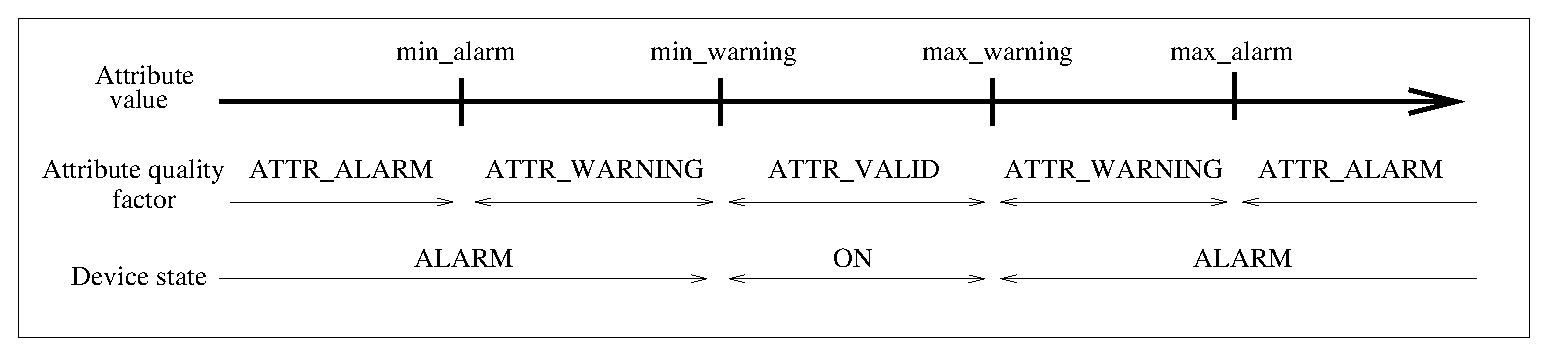
\includegraphics[scale=0.5]{advanced/alarm}
\par\end{centering}

\protect\caption{Level alarm}
\label{alarm_fig}
\end{figure}


If the min\_warning and max\_warning parameters are not set, the attribute
quality factor will simply change between Tango::ATTR\_ALARM and Tango::ATTR\_VALID
function of the attribute value.


\subsection{The Read Different than Set (RDS) alarm}

This alarm is defined only for attribute of the Tango::READ\_WRITE
and Tango::READ\_WITH\_WRITE read/write type and for numerical data
type. When the attribute is read (or when the device state is requested),
if the difference between its read value and the last written value
is something more than or equal to an authorized delta and if at least
a certain amount of milli seconds occurs since the last write operation,
the attribute quality factor will be set to Tango::ATTR\_ALARM\index{ATTR-ALARM}
and if the device state is Tango::ON, it is switched to Tango::ALARM\index{ALARM}.
If the attribute is a spectrum or an image, then the alarm is set
if any one of the attribute value's satisfies the above criterium.
This alarm configuration is done with two attribute configuration
parameters called \textbf{delta\_val\index{delta-val}} and \textbf{delta\_t\index{delta-t}}.
By default, these two parameters are not defined and no check will
be done.


\section{Enumerated\index{Enumeration} attribute}

Since Tango release 9, enumerated attribute is supported using the
new data type DevEnum\index{DevEnum}. This data type is not a real
C++ enumeration because:
\begin{enumerate}
\item The enumerated value allways start with 0
\item Values are consecutive
\item It is transferred on the network as DevShort data type
\end{enumerate}
One enumeration label is associated to each enumeration value. For
the Tango kernel, it is this list of enumeration labels which will
define the possible enumeration values. For instance if the enumeration
has 3 labels, its value must be between 0 and 2. There are two ways
to define the enumeration labels:
\begin{enumerate}
\item At attribute creation time. This is the most common case when the
list of possible enumeration values and labels are known at compile
time. The Tango code generator Pogo generates for you the code needed
to pass the enumeration labels to the Tango kernel.
\item In the user code when the enumeration values and labels are not known
at compile time but retrieved during device startup phase. The user
gives the possible enumeration values to the Tango kernel using the
Attribute class \emph{set\_properties()} method.
\end{enumerate}
A Tango client is able to retrieve the enumeration labels in the attribute
configuration returned by instance by a call to the \emph{DeviceProxy::get\_attribute\_config()}
method. Using the \emph{DeviceProxy::set\_attribute\_config()} call,
a user may change the enumeration labels but not their number.


\subsection{Usage in a Tango class}

Within a Tango class, you set the attribute value with a C++ enum
or a DevShort variable. In case a DevShort variable is used, its value
will be checked according to the enumeration labels list given to
Tango kernel.


\subsubsection{Setting the labels with enumeration compile time knowledge}

In such a case, the enumeration labels are given to Tango at the attribute
creation time in the \emph{attribute\_factory} method of the XXXClass
class. Let us take one example


\begin{minted}[linenos]{cpp}
     1  enum class Card: short
     2  {
     3      NORTH = 0,
     4      SOUTH,
     5      EAST,
     6      WEST
     7  };
     8 
     9  void XXXClass::attribute_factory(vector<Tango::Attr *> &att_list)
    10  {
    11      .....
    12      TheEnumAttrib	*theenum = new TheEnumAttrib();
    13      Tango::UserDefaultAttrProp theenum_prop;
    14      vector<string> labels = {"North","South","East","West"};
    15      theenum_prop.set_enum_labels(labels);
    16      theenum->set_default_properties(theenum_prop);
    17      att_list.push_back(theenum);
    18      .....
    19   }	
\end{minted}


line 1-7 : The definition of the enumeration (C++11 in this example)

line 14 : A vector of strings with the enumeration labels is created.
Because there is no way to get the labels from the enumeration definition,
they are re-defined here.

line 15 : This vector is given to the theenum\_prop object which contains
the user default properties

line 16 : The user default properties are associated to the attribute\\


In most cases, all this code will be automatically generated by the
Tango code generator Pogo. It is given here for completness.


\subsubsection{Setting the labels without enumeration compile time knowledge}

In such a case, the enumeration labels are retrieved by the user in
a way specific to the device and passed to Tango using the Attribute
class \emph{set\_properties()} method. Let us take one example


\begin{minted}[linenos]{cpp}
     1  void MyDev::init_device()
     2  {
     3      ...
     4  
     5      Attribute &att = get_device_attr()->get_attr_by_name("TheEnumAtt");
     6      MultiAttrProp<DevEnum> multi_prop;
     7      att.get_properties(multi_prop);
     8 
     9      multi_prop.enum_labels = {....};
    10      att.set_properties(multi_prop);
    11      ....
    12   }	
\end{minted}


line 5 : Get a reference to the attribute object

line 7 : Retrieve the attribute properties

line 9 : Initialise the attribute labels in the set of attribute properties

line 10 : Set the attribute properties


\subsubsection{Setting the attribute value}

It is possible to set the attribute value using either a classical
DevShort variable or using a variable of the C++ enumeration. The
following example is when you have compile time knowledge of the enumeration
definition. We assume that the enumeration is the same than the one
defined above (Card enumeration)


\begin{minted}[linenos]{cpp}
     1  enum Card points;
     2  
     3  void MyDev::read_TheEnum(Attribute &att)
     4  {
     5      ...
     6      points = SOUTH;
     7      att.set_value(&points);
     8  }
\end{minted}


line 1 : One instance of the Card enum is created (named points)

line 6 : The enumeration is initialized

line 7 : The value of the attribute object is set using the enumeration
(by pointer)\\
To get the same result using a classical DevShort variable, the code
looks like


\begin{minted}[linenos]{cpp}
     1  DevShort sh;
     2  
     3  void MyDev::read_TheEnum(Attribute &att)
     4  {
     5      ...
     6      sh = 1;
     7      att.set_value(&sh);
     8  }
\end{minted}


line 1 : A DevShort variable is created (named sh)

line 6 : The variable is initialized

line 7 : The value of the attribute object is set using the DevShort
variable (by pointer)


\subsection{Usage in a Tango client}

Within a Tango client, you insert/extract enumerated attribute value
in/from DeviceAttribute object with a C++ enum or a DevShort variable.
The later case is for generic client which do not have compile time
knowledge of the enumeration. The code looks like


\begin{minted}[linenos]{cpp}
     1  DeviceAttribute da = the_dev.read_attribute("TheEnumAtt");
     2  Card ca;
     3  da >> ca;
     4  
     5  DeviceAttribute db = the_dev.read_attribute("TheEnumAtt");
     6  DevShort sh;
     7  da >> sh;
\end{minted}


line 2-3 : The attribute value is extracted in a C++ enumeration variable

line 6-7 : The attribute value is extracted in a DevShort variable


\section{Device polling}


\subsection{Introduction}

Each tango device server automatically have a separate polling\index{polling}
thread pool. Polling a device means periodically executing command
on a device (or reading device attribute) and storing the results
(or the thrown exception) in a polling buffer. The aim of this polling
is threefold :
\begin{itemize}
\item Speed-up response time for slow device
\item Get a first-level history of device command output or attribute value
\item Be the data source for the Tango event system
\end{itemize}
Speeding-up response time is achieved because the command\_inout or
read\_attribute CORBA operation is able to get its data from the polling
buffer or from the a real access to the device. For ``slow'' device,
getting the data from the buffer is much faster than accessing the
device. Returning a first-level command output history (or attribute
value history) to a client is possible due to the polling buffer which
is managed as a circular buffer. The history is the contents of this
circular buffer. Obviously, the history depth is limited to the depth
of the circular buffer. The polling is also the data source for the
event system because detecting an event means being able to regularly
read the data, memorize it and declaring that it is an event after
some comparison with older values.

Starting with Tango 9, the default polling algorithm has been modifed.
However, it is still possible to use the polling as it was in Tango
releases prior to release 9. See chaper on polling configuration to
get details on this.


\subsection{Configuring the polling system}


\subsubsection{Configuring what has to be polled and how}

It is possible to configure the polling in order to poll :
\begin{itemize}
\item Any command which does not need input parameter
\item Any attribute
\end{itemize}
Configuring the polling is done by sending command to the device server
administration device automatically implemented in every device server
process. Seven commands are dedicated to this feature. These commands
are
\begin{description}
\item [{AddObjPolling\index{AddObjPolling}}] It add a new object (command
or attribute) to the list of object(s) to be polled. It is also with
this command that the polling period is specified.
\item [{RemObjPolling\index{RemObjPolling}}] To remove one object (command
or attribute) from the polled object(s) list
\item [{UpdObjPollingPeriod\index{UpdObjPollingPeriod}}] Change one object
polling period
\item [{StartPolling\index{StartPolling}}] Starts polling for the whole
process
\item [{StopPolling\index{StopPolling}}] Stops polling for the whole process
\item [{PolledDevice\index{PolledDevice}}] Allow a client to know which
device are polled
\item [{DevPollStatus\index{DevPollStatus}}] Allow a client to precisely
knows the polling status for a device
\end{description}
All the necessary parameters for the polling configuration are stored
in the Tango database. Therefore, the polling configuration is not
lost after a device server process stop and restart (or after a device
server process crash!!).

It is also possible to automatically poll a command (or an attribute)
without sending command to the device server administration device.
This request some coding (a method call) in the device server software
during the command or attribute creation. In this case, for every
devices supporting this command or this attribute, polling configuration
will be automatically updated in the database and the polling will
start automatically at each device server process startup. It is possible
to stop this behavior on a device basis by sending a RemObjPolling\index{RemObjPolling}
command to the device server administration device. The following
piece of code shows how the source code should be written.


\begin{minted}[linenos]{cpp}
     1  
     2  void DevTestClass::command_factory()
     3  {
     4  ...
     5      command_list.push_back(new IOStartPoll("IOStartPoll",
     6                                              Tango::DEV_VOID,
     7                                              Tango::DEV_LONG,
     8                                              "Void",
     9                                              "Constant number"));
    10      command_list.back()->set_polling_period(400);
    11  ...
    12  }
    13  
    14  
    15  void DevTestClass::attribute_factory(vector<Tango::Attr *> &att_list)
    16  {
    17  ...
    18      att_list.push_back(new Tango::Attr("String_attr",
    19                                          Tango::DEV_STRING,
    20                                          Tango::READ));
    21      att_list.back()->set_polling_period(250);
    22  ...
    23  }
\end{minted}


A polling period of 400 mS is set for the command called ``IOStartPoll''
at line 10 with the \emph{set\_polling\_period} method of the Command
class. Therefore, for a device of this class, the polling thread will
start polling its IOStartPoll command at process start-up except if
a RemObjPolling indicating this device and the IOStartPoll command
has already been received by the device server administration device.
This is exactly the same behavior for attribute. The polling period
for attribute called ``String\_attr'' is defined at line 20.

Configuring the polling means defining device attribute/command polling
period. The polling period has to be chosen with care. If reading
an attribute needs 200 mS, there is no point to poll this attribute
with a polling period equal or even below 200 mS. You should also
take into account that some \textquotedbl{}free\textquotedbl{} time
has to be foreseen for external request(s) on the device. On average,
for one attribute needing X mS as reading time, define a polling period
which is equal to 1.4 X (280 mS for our example of one attribute needing
200 mS as reading time). In case the polling tuning is given to external
user, Tango provides a way to define polling period minimun threshold.
This is done using device properties. These properties are named \emph{min\_poll\_period},
\emph{cmd\_min\_poll\_period} and \emph{attr\_min\_poll\_period}.
The property min\_poll\_period\index{min-poll-period} (mS) defined
a minimun polling period for the device. The property cmd\_min\_poll\_period\index{cmd-min-poll-period}
allows the definition of a minimun polling period for a specific device
command. The property attr\_min\_poll\_period\index{attr-min-poll-period}
allows the definition of a minimun polling period for one device attribute.
In case these properties are defined, it is not possible to poll the
device command/attribute with a polling period below those defined
by these properties. See Appendix A on device parameter to get a precise
syntax description for these properties.

The Jive\cite{Jive doc} tool also allows a graphical device polling
configuration.


\subsubsection{Configuring the polling threads pool}

Starting with Tango release 7, a Tango device server process may have
several polling threads managed as a pool. For instance, this could
be usefull in case of devices within the same device server process
but accessed by different hardware channel when one of the channel
is not responding (Thus generating long timeout and de-synchronising
the polling thread). By default, the polling threads pool size is
set to 1 and all the polled object(s) are managed by the same thread
(idem polling system in Tango releases older than release 7) . The
configuration of the polling thread pool is done using two properties
associated to the device server administration device. These properties
are named:
\begin{itemize}
\item \emph{polling\_threads\_pool\_size\index{polling-threads-pool-size}}
defining the maximun number of threads that you can have in the pool
\item \emph{polling\_threads\_pool\_conf\index{polling-threads-pool-conf}}
defining which threads in the pool manages which device
\end{itemize}
The granularity of the polling threads pool tuning is the device.
You cannot ask the polling threads pool to have thread number 1 in
charge of attribute \emph{att1} of device \emph{dev1} and thread number
2 to be in charge of \emph{att2} of the same device \emph{dev1}.

When you require a new object (command or attribute) to be polled,
two main cases may arrive:
\begin{enumerate}
\item Some polled object(s) belonging to the device are already polled by
one of the polling threads in the pool: There is no new thread created.
The object is simply added to the list of objects to be polled for
the existing thread
\item There is no thread already created for the device. We have two sub-cases:

\begin{enumerate}
\item The number of polling threads is less than the polling\_threads\_pool\_size:
A new thread is created and started to poll the object (command or
attribute)
\item The number of polling threads is already equal to the polling\_threads\_pool\_size:
The software search for the thread with the smallest number of polled
objects and add the new polled object to this thread
\end{enumerate}
\end{enumerate}
Each time the polling threads pool configuration is changed, it is
written in the database using the polling\_threads\_pool\_conf property.
If the behaviour previously described does not fulfill your needs,
it is possible to update the polling\_threads\_pool\_conf property
in a graphical way using the Tango Astor \cite{Astor_doc} tool or
manually using the Jive tool \cite{Jive doc}. These changes will
be taken into account at the next device server process start-up.
At start-up, the polling threads pool will allways be configured as
required by the polling\_threads\_pool\_conf property. The syntax
used for this property is described in the Reference part of the Appendix
\ref{cha:Reference-part}. The following window dump is the Astor
tool window which allows polling threads pool management.\begin{center}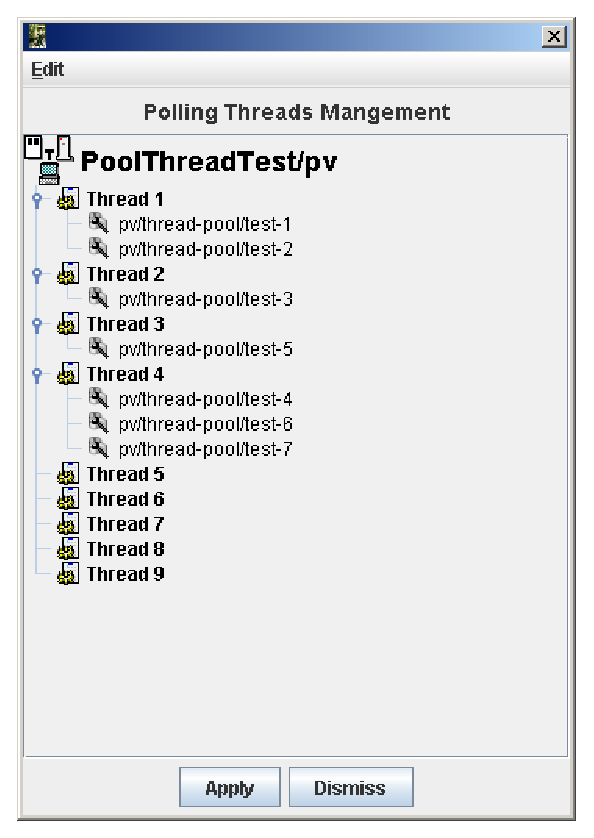
\includegraphics{advanced/ThreadsManagement}\end{center}

In this example, the polling threads pool size to set to 9 but only
4 polling threads are running. Thread 1 is in charge of all polled
objects related to device pv/thread-pool/test-1 and pv/thread-pool/test-2.
Thread 2 is in charge of all polled objects related to device pv/thread-pool/test-3.
Thread 3 is in charge of all polled objects related to device pv/thread-pool/test-5
anf finally, thread 4 is in charge of all polled objects for devices
pv/thread-pool/test-4, pv/thread-pool/test-6 and pv/thread-pool/test-7.

It's also possible to define the polling threads pool size programmatically
in the main function of a device server process using the \emph{Util::set\_polling\_threads\_pool\_size()\index{set-polling-threads-pool-size}}
method before the call to the \emph{Util::server\_init()} method


\subsubsection{Choosing polling algorithm}

Starting with Tango 9, you can choose between two different polling
algorithm:
\begin{itemize}
\item The polling as it was in Tango since it has been introduced. This
means:

\begin{itemize}
\item For one device, always poll attribute one at a time even if the polling
period is the same (use of read\_attribute instead of read\_attributes)
\item Do not allow the polling thread to be late: If it is the case (because
at the end of polling object 1, the time is greater than the polling
date of object 2), discard polling object and inform event user by
sending one event with error (Polling thread is late and discard....)
\end{itemize}
\item New polling algorithm introduced in Tango 9 as the default one. This
means:

\begin{itemize}
\item For one device, poll all attributes with the same polling period using
a single device call (read\_attributes)
\item Allow the polling thread to be late but only if number of late objects
decreases.
\end{itemize}
\end{itemize}
The advantages of new polling algorithm are 
\begin{enumerate}
\item In case of several attributes polled on the same device at the same
period a lower device occupation time by the polling thread (due to
a single read\_attributes() call instead of several single read\_attribute()
calls)
\item Less ``Polling thread late'' errors in the event system in case
of device with non constant response time
\end{enumerate}
The drawback is
\begin{enumerate}
\item The loss of attribute individual timing data reported in the polling
thread status
\end{enumerate}
It is still possible to return to pre-release 9 polling algorithm.
To do so, you can use the device server process administration device
\emph{polling\_before\_9}\index{polling_before_9@polling\_before\_9}
property by setting it to true. It is also possible to choose this
pre-release 9 algorithm in device server process code in the main
function of the process using the \emph{Util::set\_polling\_before\_9()}
method.


\subsection{Reading data from the polling buffer}

For a polled command or a polled attribute, a client has three possibilities
to get command result or attribute value (or the thrown exception)
:
\begin{itemize}
\item From the device itself
\item From the polling buffer
\item From the polling buffer first and from the device if data in the polling
buffer are invalid or if the polling is badly configured.
\end{itemize}
The choice is done during the command\_inout CORBA operation by positioning
one of the operation parameter. When reading data from the polling
buffer, several error cases are possible 
\begin{itemize}
\item The data in the buffer are not valid any more. Every time data are
requested from the polling buffer, a check is done between the client
request date and the date when the data were stored in the buffer.
An exception is thrown if the delta is greater than the polling period
multiplied by a ``too old'' factor. This factor has a default value
and is up-datable via a device property. This is detailed in the reference
part of this manual.
\item The polling is correctly configured but there is no data yet in the
polling buffer.
\end{itemize}

\subsection{Retrieving command/attribute result history}

The polling thread stores the command result or attribute value in
circular buffers. It is possible to retrieve an history of the command
result (or attribute value) from these polling buffers. Obviously
the history is limited by the depth of the circular buffer. For commands,
a CORBA operation called \emph{command\_inout\_history\_2\index{command-inout-history-2}}
allows this retrieval. The client specifies the command name and the
record number he want to retrieve. For each record, the call returns
the date when the command was executed, the command result or the
exception stack in case of the command failed when it was executed
by the polling thread. In such a case, the exception stack is sent
as a structure member and not as an exception. The same thing is available
for attribute. The CORBA operation name is \emph{read\_attribute\_history\_2\index{read-attribute-history-2}.}
For these two calls, there is no check done between the call date
and the record date in contrary of the call to retrieve the last command
result (or attribute value).


\subsection{Externally triggered polling}

Sometimes, rather than polling a command or an attribute regulary
with a fixed period, it is more interesting to \textquotedbl{}manually\textquotedbl{}
decides when the polling must occurs. The Tango polling system also
supports this kind of usage. This is called \emph{externally triggered
polling}. To define one attribute (or command) as externally triggered,
simply set its polling period to 0. This can be done with the device
server administration device AddObjPolling or UpdObjPollingPeriod
command. Once in this mode, the attribute (or command) polling is
triggered with the \emph{trigger\_cmd\_polling()} method (or \emph{trigger\_attr\_polling()}
method) of the Util class. The following piece of code shows how this
method could be used for one externally triggered command.


\begin{minted}[linenos]{cpp}
     1  .....
     2  
     3  string ext_polled_cmd("MyCmd");
     4  Tango::DeviceImpl *device = .....;
     5  
     6  Tango::Util *tg = Tango::Util::instance();
     7  
     8  tg->trigger_cmd_polling(device,ext_polled_cmd);
     9  
    10  .....

\end{minted}


line 3 : The externally polled command name

line 4 : The device object

line 8 : Trigger polling of command MyCmd


\subsection{Filling polling buffer}

Some hardware to be interfaced already returned an array of pair value,
timestamp. In order to be read with the \emph{command\_inout\_history}
or \emph{read\_attribute\_history} calls, this array has to be transferred
in the attribute or command polling buffer. This is possible only
for attribute or command configured in the externally triggered polling
mode. Once in externally triggered polling mode, the attribute (or
command) polling buffer is filled with the \emph{fill\_cmd\_polling\_buffer()\index{fill-cmd-polling-buffer}}
method (or \emph{fill\_attr\_polling\_buffer()\index{fill-attr-polling-buffer}}
method) of the Util class. For command, the user uses a template class
called \emph{TimedCmdData\index{TimedCmdData}} for each element of
the command history. Each element is stored in a stack in one instance
of a template class called \emph{CmdHistoryStack\index{CmdHistoryStack}.}
This object is one of the argument of the fill\_cmd\_polling\_buffer()
method. Obviously, the stack depth cannot be larger than the polling
buffer depth. See \ref{sub:The-device-polling-prop} to learn how
the polling buffer depth is defined. The same way is used for attribute
with the \emph{TimedAttrData\index{TimedAttrData}} and \emph{AttrHistoryStack\index{AttrHistoryStack}}
template classes. These classes are documented in \cite{TANGO_ref_man}.
The following piece of code fills the polling buffer for a command
called MyCmd which is already in externally triggered mode. It returns
a DevVarLongArray data type with three elements. This example is not
really something you will find in a real hardware interface. It is
only to demonstrate the fill\_cmd\_polling\_buffer() method usage.
Error management has also been removed.


\begin{minted}[linenos]{cpp}
     1  ....
     2  
     3  Tango::DevVarLongArray dvla_array[4];
     4          
     5  for(int i = 0;i < 4;i++)
     6  {
     7      dvla_array[i].length(3);
     8      dvla_array[i][0] = 10 + i;
     9      dvla_array[i][1] = 11 + i;
    10      dvla_array[i][2] = 12 + i;
    11  }
    12  
    13  Tango::CmdHistoryStack<DevVarLongArray> chs;
    14  chs.length(4);
    15  
    16  for (int k = 0;k < 4;k++)
    17  {
    18      time_t when = time(NULL);
    19  
    20      Tango::TimedCmdData<DevVarLongArray> tcd(&dvla_array[k],when);
    21      chs.push(tcd);
    22  }
    23  
    24  Tango::Util *tg = Tango::Util::instance();
    25  string cmd_name("MyCmd");
    26  DeviceImpl *dev = ....;
    27  
    28  tg->fill_cmd_polling_buffer(dev,cmd_name,chs);
    29  
    30  .....

\end{minted}


Line 3-11 : Simulate data coming from hardware

Line 13-14 : Create one instance of the CmdHistoryStack class and
reserve space for one history of 4 elements

Line 16-17 : A loop on each history element

Line 18 : Get date (hardware simulation)

Line 20 : Create one instance of the TimedCmdData class with data
and date

Line 21 : Store this command history element in the history stack.
The element order will be the insertion order whatever the element
date is.

Line 28 : Fill command polling buffer

After one execution of this code, a command\_inout\_history() call
will return one history with 4 elements. The first array element of
the oldest history record will have the value 10. The first array
element of the newest history record will have the value 13. A command\_inout()
call with the data source parameter set to CACHE will return the newest
history record (ie an array with values 13,14 and 15). A command\_inout()
call with the data source parameter set to DEVICE will return what
is coded is the command method. If you execute this code a second
time, a command\_inout\_history() call will return an history of 8
elements.

The next example fills the polling buffer for an attribute called
MyAttr which is already in externally triggered mode. It is a scalar
attribute of the DevString data type. This example is not really something
you will find in a real hardware interface. It is only to demonstrate
the fill\_attr\_polling\_buffer() method usage with memory management
issue. Error management has also been removed.


\begin{minted}[linenos]{cpp}
     1  ....
     2  
     3  AttrHistoryStack<DevString> ahs;
     4  ahs.length(3);
     5  
     6  for (int k = 0;k < 3;k++)
     7  {
     8      time_t when = time(NULL);
     9  
    10      DevString *ptr = new DevString [1];
    11      ptr = CORBA::string_dup("Attr history data");
    12  
    13      TimedAttrData<DevString> tad(ptr,Tango::ATTR_VALID,true,when);
    14      ahs.push(tad);
    15  }
    16  
    17  Tango::Util *tg = Tango::Util::instance();
    18  string attr_name("MyAttr");
    19  DeviceImpl *dev = ....;
    20  
    21  tg->fill_attr_polling_buffer(dev,attr_name,ahs);
    22  
    23  .....
  
\end{minted}


Line 3-4 : Create one instance of the AttrHistoryStack class and reserve
space for an history with 3 elements

Line 6-7 : A loop on each history element

Line 8 : Get date (hardware simulation)

Line 10-11 : Create a string. Note that the DevString object is created
on the heap

Line 13 : Create one instance of the TimedAttrData class with data
and date requesting the memory to be released.

Line 14 : Store this attribute history element in the history stack.
The element order will be the insertion order whatever the element
date is.

Line 21 : Fill command polling buffer

It is not necessary to return the memory allocated at line 10. The
\emph{fill\_attr\_polling\_buffer()} method will do it for you.


\subsection{Setting and tuning the polling in a Tango class}

Even if the polling is normally set and tuned with external tool like
Jive, it is possible to set it directly into the code of a Tango class.
A set of methods belonging to the \emph{DeviceImpl} class allows the
user to deal with polling. These methods are:
\begin{itemize}
\item \emph{is\_attribute\_polled()} and \emph{is\_command\_polled()} to
check if one command/attribute is polled
\item \emph{get\_attribute\_poll\_period()} and \emph{get\_command\_poll\_period()}
to get polled object polling period
\item \emph{poll\_attribute()} and \emph{poll\_command()} to poll command
or attribute
\item \emph{stop\_poll\_attribute()} and \emph{stop\_poll\_command()} to
stop polling a command or an attribute
\end{itemize}
The following code snippet is just an exmaple of how these methods
could be used. They are documented in \cite{Tango-dsclasses-doc}


\begin{minted}[linenos]{cpp}
     [Program Listing: poll_in_ds.cpp.lines
     1	void MyClass::read_attr(Tango::Attribute &attr)
     2	{
     3	    ...
     4	    ...
     5	    
     6	    string att_name("SomeAttribute");
     7	    string another_att_name("AnotherAttribute");
     8	
     9	    if (is_attribute_polled(att_name) == true)
    10	        stop_poll_attribute(att_name);
    11	    else
    12	        poll_attribute(another_att_name,500); 
    13	    
    14	    ....
    15	    ....
    16	    
    17	}

]
\end{minted}



\section{Threading}
\label{sec:Threading}

When used with C++, Tango used omniORB as underlying ORB. This CORBA
implementation is a threaded implementation and therefore a C++ Tango
device server or client are multi-threaded processes.


\subsection{Device server process}

A classical Tango device server without any connected clients has
eight threads. These threads\index{thread} are :
\begin{itemize}
\item The main thread waiting in the ORB main loop
\item Two ORB implementation threads (the POA thread)
\item The ORB scavanger thread
\item The signal thread
\item The heartbeat thread (needed by the Tango event system)
\item Two Zmq implementation threads
\end{itemize}
On top of these eight threads, you have to add the thread(s) used
by the polling threads pool. This number depends on the polling thread
pool configuration and could be between 0 (no polling at all) and
the maximun number of threads in the pool.

A new thread is started for each connected client. Device server are
mostly used to interface hardware which most of the time does not
support multi-threaded access. Therefore, all remote calls executed
from a client are serialized within the device server code by using
mutual exclusion. See chapter \ref{sub:Serialization-model-within}
on which serialization model are available. In order to limit thread
number, the underlying ORB (omniORB) is configured to shutdown threads
dedicated to client if the connection is inactive for more than 3
minutes. To also limit thread number, the ORB is configured to create
one thread per connection up to 55 threads. When this level is reached,
the threading model is automatically switch to a \textquotedbl{}thread
pool\textquotedbl{} model with up to 100 threads. If the number of
threads decrease down to 50, the threading model will return to \textquotedbl{}thread
per connection\textquotedbl{} model.

If you are using event, the event system for its internal heartbeat
system periodically (every 200 seconds) sends a command to the device
server administration device. As explained above, a thread is created
to execute these command. The omniORB scavanger will terminate this
thread before the next event system heartbeat command arrives. For
example, if you have a device server with three connected clients
using only event, the process thread number will permanently change
between 8 and 11 threads.

In summary, the number of threads in a device server process can be
evaluated with the following formula:\begin{center}\textbf{8 + k
+ m}\end{center}k is the number of polling threads used from the
polling threads pool and m is the number of threads used for connected
clients.


\subsubsection{Serialization model within a device server}
\label{sub:Serialization-model-within}

Four serialization\index{serialization} models are available within
a device server. These models protect all requests coming from the
network but also requests coming from the polling thread. These models
are:
\begin{enumerate}
\item Serialization by device. All access to the same device are serialized.
As an example, let's take a device server implementing one class of
device with two instances (dev1 and dev2). Two clients are connected
to these devices (client1 and client2). Client2 will not be able to
access dev1 if client1 is using it. Nevertheless, client2 is able
to access dev2 while client1 access dev1 (There is one mutual exclusion
object by device)
\item Serialization by class. With non multi-threaded legacy software, the
preceding scenario could generate problem. In this mode of serialization,
client2 is not able to access dev2 while client1 access dev1 because
dev2 and dev1 are instances of the same class (There is one mutual
exclusion object by class)
\item Serialization by process. This is one step further than the previous
case. In this mode, only one client can access any device embedded
within the device server at a time. There is only one mutual exclusion
object for the whole process)
\item No serialization. This is an exotic kind of serialization and \textbf{should
be used with extreme care} only with device which are fully thread
safe. In this model, most of the device access are not serialized
at all. Due to Tango internal structure, the \emph{get\_attribute\_config},
\emph{set\_attribute\_config}, \emph{read\_attributes} and \emph{write\_attributes}
CORBA calls are still protected. Reading the device state and status
via commands or via CORBA attribute is also protected.
\end{enumerate}
By default, every Tango device server is in serialization by device
mode. A method of the Tango::Util class allows to change this default
behavior.\newpage{}


\begin{minted}[linenos]{cpp}
     1  #include <tango.h>
     2  
     3  int main(int argc,char *argv[])
     4  {
     5  
     6      try
     7      {
     8          
     9          Tango::Util *tg = Tango::Util::init(argc,argv);
    10  
    11          tg->set_serial_model(Tango::BY_CLASS);
    12  
    13          tg->server_init();
    14  
    15          cout << "Ready to accept request" << endl;
    16          tg->server_run();
    17      }
    18      catch (bad_alloc)
    19      {
    20           cout << "Can't allocate memory!!!" << endl;
    21           cout << "Exiting" << endl;
    22      }
    23      catch (CORBA::Exception &e)
    24      {
    25           Tango::Except::print_exception(e);
    26                  
    27           cout << "Received a CORBA::Exception" << endl;
    28           cout << "Exiting" << endl;
    29      }
    30          
    31      return(0);
    32  }

\end{minted}


The serialization model is set at line 11 before the server is initialized
and the infinite loop is started. See \cite{TANGO_ref_man} for all
details on the methods to set/get serialization model.


\subsubsection{Attribute Serialization model}

Even with the serialization model described previously, in case of
attributes carrying a large number of data and several clients reading
this attribute, a device attribute serialization has to be followed.
Without this level of serialization, for attribute using a shared
buffer, a thread scheduling may happens while the device server process
is in the CORBA layer transferring the attribute data on the network.
Three serialization\index{serialization} models are available for
attribute serialization. The default is well adapted to nearly all
cases. Nevertheless, if the user code manages several attributes data
buffer or if it manages its own buffer protection by one way or another,
it could be interesting to tune this serialization level. The available
models are:
\begin{enumerate}
\item Serialization by kernel. This is the default case. The kernel is managing
the serialization
\item Serialization by user. The user code is in charge of the serialization.
This serialization is done by the use of a omni\_mutex object. An
omni\_mutex is an object provided by the omniORB package. It is the
user responsability to lock this mutex when appropriate and to give
this mutex to the Tango kernel before leaving the attribute read method
\item No serialization.
\end{enumerate}
By default, every Tango device attribute is in serialization by kernel.
Methods of the Tango::Attribute class allow to change the attribute
serialization behavior and to give the user omni\_mutex object to
the kernel.


\begin{minted}[linenos]{cpp}
1 void MyClass::init_device()
2 {
3    ...
4    ...
5    Tango::Attribute &att = dev_attr->get_attr_by_name("TheAttribute");
6    att.set_attr_serial_model(Tango::ATTR_BY_USER);
7    ....
8    ....
9 
10 }
11 
12 
13 void MyClass::read_TheAttribute(Tango::Attribute &attr)
14 {
15    ....
16    ....
17    the_mutex.lock();
18    ....
19    // Fill the attribute buffer
20    ....
21    attr.set_value(buffer,....);
22    attr->set_user_attr_mutex(&the_mutex);
23 }
24 
\end{minted}


The serialization model is set at line 6 in the init\_device() method.
The user omni\_mutex is passed to the Tango kernel at line 22. This
omni\_mutex object is a device data member. See \cite{TANGO_ref_man}
for all details on the methods to set attribute serialization model.


\subsection{Client process}

Clients are also multi threaded processes. The underlying C++ ORB
(omniORB) try to keep system resources to a minimum. To decrease process
file descriptors usage, each connection to server is automatically
closed if it is idle for more than 2 minutes and automatically re-opened
when needed. A dedicated thread is spawned by the ORB to manage this
automatic closing connection (the ORB scavenger thread).

Threrefore, a Tango client has two threads which are:
\begin{enumerate}
\item The main thread
\item The ORB scavanger thread
\end{enumerate}
If the client is using the event system and as Tango is using the
event push-push model, it has to be a server for receiving the events.
This increases the number of threads\index{thread}. The client now
has 6 threads which are:
\begin{itemize}
\item The main thread
\item The ORB scavenger thread
\item Two Zmq implementation threads
\item Two Tango event system related threads (the KeepAliveThread and the
EventConsumer thread)
\end{itemize}

\section{Generating events in a device server}

The server is at the origin of events\index{event}. It will fire
events as soon as they occur. Standard events (\emph{change}, \emph{periodic}
and \emph{archive}) are detected automatically in the polling thread
and fired as soon as they are detected. The \emph{periodic} events
can only be handled by the polling thread. \emph{Change, Data ready}
and \emph{archive} events can also be pushed from the device server
code. To allow a client to subscribe to events of non polled attributes
the server has to declare that events are pushed from the code. Three
methods are available for this purpose:
\begin{minted}[linenos]{cpp}
Attr::set_change_event(bool implemented, bool detect = true);
Attr::set_archive_event(bool implemented, bool detect = true);
Attr::set_data_ready_event( bool implemented);
\end{minted}
where \emph{implemented}=true indicates that events are pushed manually
from the code and \emph{detect}=true (when used) triggers the verification
of the same event properties as for events send by the polling thread.
When setting \emph{detect}=false, no value checking is done on the
pushed value! The class DeviceImpl also supports the first two methods
with an addictional parameter attr\_name defining the attribute name.

To push events manually from the code a set of data type dependent
methods can be used:
\begin{minted}[linenos]{cpp}
DeviceImpl::push_change_event (string attr_name, ....);
DeviceImpl::push_archive_event(string attr_name, ....);
\end{minted}
For the data ready event, a DeviceImpl class method has to be used
to push the event.
\begin{minted}[linenos]{cpp}
DeviceImpl::push_data_ready_event(string attr_name,Tango::DevLong ctr);
\end{minted}
See the class documentation for all available interfaces.

For non-standard events a single call exists for pushing the data
to the CORBA Notification Service (omniNotify). Clients who are subscribed
to this event have to know what data type is in the DeviceAttribute
and unpack it accordingly.

To push non-standard events, use the following api call is available
to all device servers :
\begin{minted}[linenos]{cpp}
DeviceImpl::push_event( string attr_name,
             vector<string> &filterable_names,
             vector<double> &filterable_vals,
             Attribute &att)
\end{minted}
where \emph{attr\_name} is the name of the attribute\emph{. Filterable\_names}
and \emph{filterable\_vals} represent any filterable data which can
be used by clients to filter on. Here is a typical example of what
a server will need to do to send its own events. We are in the read
method of the \textquotedbl{}Sinusoide\textquotedbl{} attribute. This
attribute is readable as any other attribute but an event is sent
if its value is positive when it is read. On top of that, this event
is sent with one filterable field called \textquotedbl{}value\textquotedbl{}
which is set to the attribute value.


\begin{minted}[linenos]{cpp}
1  void MyClass::read_Sinusoide(Tango::Attribute &attr)
2  {
3    ...
4       struct timeval tv;
5       gettimeofday(&tv, NULL);
6       sinusoide = 100 * sin( 2 * 3.14 * frequency * tv.tv_sec);
7  
8       if (sinusoide >= 0) 
9       {
10          vector<string> filterable_names;
11          vector<double> filterable_value;
12 
13          filterable_names.push_back("value");
14          filterable_value.push_back((double)sinusoide);
15 
16          push_event( attr.get_name(),
17                      filterable_names, filterable_value,
18                      &sinusoide);
19       }
20    ....
21    ....
22 
23 }
\end{minted}


line 13-14 : The filter pair name/value is initialised

line 16-18 : The event is pushed


\section{Using multicast protocol to transfer events}

This feature is available starting with Tango 8.1. Transferring events
using a multicast\index{multicasting} protocol means delivering the
events to a group of clients simultaneously in a single transmission
from the event source. Tango, through ZMQ, uses the OpenPGM multicating
protocol. This is one implementation of the PGM protocol defined by
the RFC 3208 (Reliable multicasting protocol). Nevertheless, the default
event communication mode is unicast and propagating events via multicasting
requires some specific configuration.


\subsection{Configuring events to use multicast transport}

Before using multicasting transport for event(s), you have to choose
which address and port have to be used. In a IP V4 network, only a
limited set of addresses are associated with multicasting. These are
the IP V4 addresses between \begin{center}224.0.1.0 and 238.255.255.255\end{center}
Once the address is selected, you have to choose a port number. Together
with the event name, these are the two minimum configuration informations
which have to be provided to Tango to get multicast transport. This
configuration is done using the \textbf{MulticastEvent\index{MulticastEvent}}
free property associated to the \textbf{CtrlSystem\index{CtrlSystem}}
object. \begin{center}

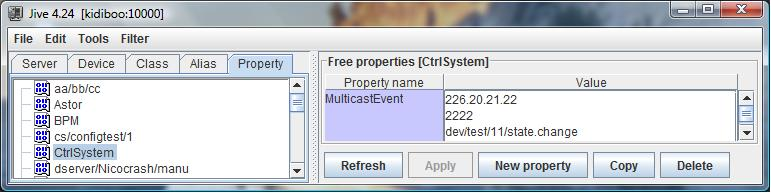
\includegraphics[scale=0.7]{advanced/jive_simpl}\end{center}

In the above window dump of the Jive tool, the \emph{change} event
on the \emph{state} attribute of the \emph{dev/test/11} device has
to be transferred using multicasting with the address \emph{226.20.21.22}
and the port number \emph{2222}. The exact definition of this CtrlSystem/MulticastEvent
property for one event propagated using multicast is


\begin{minted}[linenos]{cpp}
1 CtrlSystem->MulticastEvent:   Multicast address,
2                               port number,
3                               [rate in Mbit/sec],
4                               [ivl in seconds],
5                               event name
\end{minted}


Rate\index{rate} and Ivl\index{ivl} are optional properties. In
case several events have to be transferred using multicasting, simply
extend the MulicastEvent property with the configuration parameters
related to the other events. There is only one MultiCastEvent property
per Tango control system. The underlying multicast protocol (PGM)
is rate limited. This means that it limits its network bandwidth usage
to a user defined value. The optional third configuration parameter
is the maximum rate (in Mbit/sec) that the protocol will use to transfert
this event. Because PGM is a reliable protocol, data has to be buffered
for re-transmission in case a receiver signal some lost data. The
optional forth configuration parameter specify the maximum amount
of time (in seconds) that a receiver can be absent for a multicast
group before unrecoverable data loss will occur. Exercise care when
setting large recovery interval as the data needed for recovery will
be held in memory. For example, a 60 seconds (1 minute) recovery interval
at a data rate of 1 Gbit/sec requires a 7 GBytes in-memory buffer.
Whan any of these two optional parameters are not set, the default
value (defined in next sub-chapter) are used. Here is another example
of events using multicasting configuration\begin{center}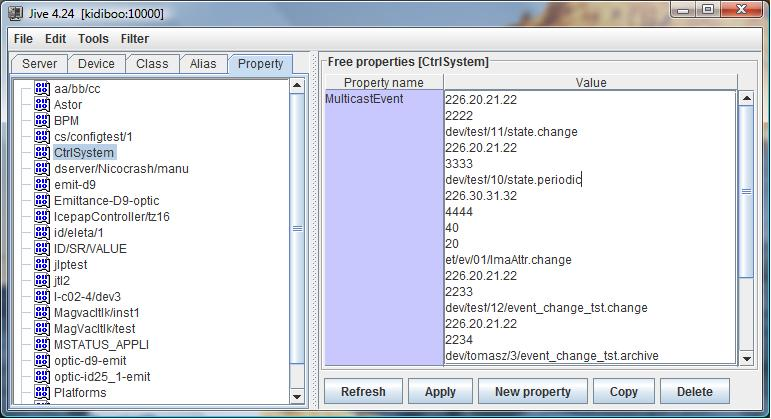
\includegraphics[scale=0.7]{advanced/jive_sophis}\end{center}
In this example, there are 5 events which are transmitted using multicasting:
\begin{enumerate}
\item Event \emph{change} for attribute \emph{state} on device \emph{dev/test/11}
which uses multicasting address \emph{226.20.21.22} and port number
\emph{2222}
\item Event \emph{periodic} for attribute \emph{state} on device \emph{dev/test/10}
which uses multicasting address \emph{226.20.21.22} and port number
\emph{3333}
\item Event \emph{change} for attribute \emph{ImaAttr} on device \emph{et/ev/01}
which uses multicasting address \emph{226.30.31.32} and port number
\emph{4444}. Note that this event uses a rate set to \emph{40 Mbit/sec}
and a ivl set to \emph{20 seconds}.
\item Event \emph{change} for attribute \emph{event\_change\_tst} on device
\emph{dev/test/12} which uses multicasting address \emph{226.20.21.22}
and port number \emph{2233}
\item Event \emph{archive} for attribute \emph{event\_change\_tst} on device
\emph{dev/tomasz/3} which uses multicasting address \emph{226.20.21.22}
and port number \emph{2234}
\end{enumerate}

\subsection{Default multicast related properties}

On top of the MulticastEvent property previously described, Tango
supports three properties to defined default value for multicast transport
tuning. These properties are:
\begin{itemize}
\item \textbf{MulticastRate}\index{MulticastRate} associated to the CtrlSystem\index{CtrlSystem}
object. This defines the maximum rate will will be used by the multicast
protocol when transferring event. The unit is Mbit/sec. In case this
property is not defined, the Tango library used a value of 80 Mbit/sec.
\item \textbf{MulticastIvl}\index{MulticastIvl} associated to the CtrlSystem
object. It specifies the maximum time (in sec) during which data has
to be buffered for re-transmission in case a receiver signals some
lost data. The unit is seconds. In case this property is not defined,
the Tango library takes a value of 20 seconds.
\item \textbf{MulticastHops}\index{MulticastHops} associated to the CtrlSystem
object. This property defines the maximum number of element (router),
the multicast packet is able to cross. Each time one element is crossed,
the value is decremented. When it reaches 0, the packet is not transferred
any more. In case this property is not defined, the Tango library
uses a value of 5.
\end{itemize}

\section{Memorized attribute}

It is possible to ask Tango to store in its database the last written
value for attribute of the SCALAR data format and obviously only for
READ\_WRITE or READ\_WITH\_WRITE attribute. This is fully automatic.
During device startup phase, for all device memorized\index{memorized}
attributes, the value written in the database is fetched and applied.
A write\_attribute call can be generated to apply the memorized value
to the attribute or only the attribute set point can be initialised.
The following piece of code shows how the source code should be written
to set an attribute as memorized and to initialise only the attribute
set point.


\begin{minted}[linenos]{cpp}
1 void DevTestClass::attribute_factory(vector<Tango::Attr *> &att_list)
2  {
3      ...
4      att_list.push_back(new String_attrAttr());
5      att_list.back()->set_memorized();
6      att_list.back()->set_memorized_init(false);
7      ...
8  }
\end{minted}


Line 4 : The attribute to be memorized is created and inserted in
the attribute vector.

Line 5 : The \emph{set\_memorized()} method of the attribute base
class is called to define the attribute as memorized.

Line 6 : The set\_memorized\_init() method is called with the parameter
false to define that only the set point should be initialsied.


\section{Forwarded attribute}


\subsection{Definition}

Let's take an example to explain what is a forwarded attribute. We
assume we have to write a Tango class for a ski lift in a ski resort
somewhere in the Alps. Obviously, the ski lift has a motor for which
we already have a Tango class. This motor Tango class has one attribute
\emph{speed}. But for the ski lift, the motor speed is not the only
thing which has to be controlled. For instance, you also want to give
access to the wind sensor data installed on the top of the ski lift.
Therefore, you write a ski-lift Tango class representing the whole
ski-lift system. This ski-lift class will have at least two attributes
which are:
\begin{enumerate}
\item The wind speed at the top of the ski-lift
\item The motor speed
\end{enumerate}
The ski-lift Tango class motor speed attribute is nothing more than
the motor Tango class speed attribute. All the ski-lift class has
to do for this attribute is to forward the request (read/write) to
the speed attribute of the motor Tango class. The speed attribute
of the ski-lift Tango class is a \textbf{forwarded attribute\index{forwarded-attribute}}
while the speed attribute of the motor Tango class is its \textbf{root
attribute}\index{root-attribute}.

A forwarded attribute get its configuration from its root attribute
and it forwards to its root attribute
\begin{itemize}
\item Its read / write / write\_read requests
\item Its configuration change
\item Its event subscription
\item Its locking behavior
\end{itemize}
As stated above, a forwarded attribute has the same configuration
than its root attribute except its \emph{name} and \emph{label} which
stays local. All other attribute configuration parameters are forwarded
to the root attribute. If a root attribute configuration parameter
is changed, the forwarded attribute is informed (via event) and its
local configuration is also modified.

The association between the forwarded attribute and its root attribute
is done using a property named \begin{center}\_\_root\_att\end{center}
belonging to the forwarded attribute. This property value is simply
the name of the root attribute. Muti-control system is supported and
this \_\_root\_att\index{__root_att@\_\_root\_att} attribute property
value can be something like \emph{tango://my\_tango\_host:10000/my/favorite/dev/the\_root\_attribute}.
The name of the root attribute is included in attribute configuration.

It is forbidden to poll a forwarded attribute and one exception is
thrown if such a case happens. Polling has to be done on the root
attribute. Nevertheless, if the root attribute is polled, a request
to read the forwarded attribute with the DeviceProxy object source
parameter set to CACHE\_DEVICE or CACHE will get its data from the
root attribute polling buffer.

If you subscribe to event(s) on a forwarded attribute, the subscription
is forwarded to the root attribute. When the event is received by
the forwarded attribute, the attribute name in the event data is modified
to reflect the forwarded attribute name and the event is pushed to
the original client(s).

When a device with forwarded attribute is locked, the device to which
the root attribute belongs is also locked.


\subsection{Coding}

As explained in the chapter \textquotedbl{}Writing a Tango device
server\textquotedbl{}, each Tango class attribute is implemented via
a C++ class which has to inherit from either \emph{Attr}, \emph{SpectrumAttr}
or \emph{ImageAttr} according to the attribute data format. For forwarded
attribute, the related class has to inherit from the \textbf{FwdAttr\index{FwdAttr}}
class whatever its data format is. For classical attribute, the programmer
can define in the Tango class code default value for the attribute
properties using one instance of the \emph{UserDefaultAttrProp} class.
For forwarded attribute, the programmer has to create one instance
of the \textbf{UserDefaultFwdAttrProp\index{UserDefaultFwdAttrProp}}
class but only the attribute label can be defined. One example of
how to program a forwarded attribute is given below


\begin{minted}[linenos]{cpp}
1  class MyFwdAttr: public Tango::FwdAttr
2  { 
3  public:     
4      MyFwdAttr(const string &_n):FwdAttr(_n) {}; 	
5      ~MyFwdAttr() {}; 
6  };
7
8  void DevTestClass::attribute_factory(vector<Tango::Attr *> &att_list)
9  {
10     ...
11     MyFwdAttr *att1 = new MyFwdAttr("fwd_att_name");
12     Tango::UserDefaultFwdAttrProp att1_prop; 	
13     att1_prop.set_label("Gasp a fwd attribute");
14     att1->set_default_properties(att1_prop); 	
15     att_list.push_back(att1);
14     ...
15  }
\end{minted}


Line 1 : The forwarded attribute class inherits from FwdAttr class.

Line 4-5 : Only constructor and destructor methods are required

Line 11 : The attribute object is created

Line 12-14 : A default value for the forwarded attribute label is
defined.

Line 15: The forwarded attribute is added to the list of attribute

In case of error in the forwarded attribute configuration (for instance
missing \_\_root\_att property), the attribute is not created by the
Tango kernel and is therefore not visible for the external world.
The state of the device to which the forwarded attribute belongs to
is set to ALARM (if not already FAULT) and a detailed error report
is available in the device status. In case a device with forwarded
attribute(s) is started before the device(s) with the root attribute(s),
the same principle is used: forwarded attribute(s) are not created,
device state is set to ALARM and device status is reporting the error.
When the device(s) with the root attribute will start, the forwarded
attributes will automatically be created. 


\section{Transferring images}

Some optimized methods have been written to optimize image transfer
between client and server using the attribute DevEncoded\index{DevEncoded}
data type. All these methods have been merged in a class called EncodedAttribute.
Within this class, you will find methods to:
\begin{itemize}
\item Encode an image in a compressed way (JPEG\index{JPEG}) for images
coded on 8 (gray scale), 24 or 32 bits
\item Encode a grey scale image coded on 8 or 16 bits
\item Encode a color image coded on 24 bits
\item Decode images coded on 8 or 16 bits (gray scale) and returned a 8
or 16 bits grey scale image
\item Decode color images transmitted using a compressed format (JPEG) and
returns a 32 bits RGB image
\end{itemize}
The following code snippets are examples of how these methods have
to be used in a server and in a client. On the server side, creates
an instance of the EncodedAttribute\index{EncodedAttribute} class
within your object


\begin{minted}[linenos]{cpp}
1 class MyDevice::Tango::Device_4Impl
2  {
3      ...
4      Tango::EncodedAttribute jpeg;
5      ...
6  }
\end{minted}


In the code of your device, use an encoding method of the EncodedAttribute
class


\begin{minted}[linenos]{cpp}
1 void MyDevice::read_Encoded_attr_image(Tango::Attribute &att)
2 {
3      ....
4      jpeg.encode_jpeg_gray8(imageData,256,256,50.0);
5      att.set_value(&jpeg);
6 }
\end{minted}


Line 4: Image encoding. The size of the image is 256 by 256. Each
pixel is coded using 8 bits. The encoding quality is defined to 50
in a scale of 0 - 100. imageData is the pointer to the image data
(pointer to unsigned char)

Line 5: Set the value of the attribute using a \emph{Attribute::set\_value()}
method.

On the client side, the code is the following (without exception management)


\begin{minted}[linenos]{cpp}
1    ....
2    DeviceAttribute da;
3    EncodedAttribute att;
4    int width,height;
5    unsigned char *gray8;
6      
7    da = device.read_attribute("Encoded_attr_image");
8    att.decode_gray8(&da,&width,&height,&gray8);
9    ....
10   delete [] gray8;
11   ...
\end{minted}


The attribute named Encoded\_attr\_image is read at line7. The image
is decoded at line 8 in a 8 bits gray scale format. The image data
are stored in the buffer pointed to by \textquotedbl{}gray8\textquotedbl{}.
The memory allocated by the image decoding at line 8 is returned to
the system at line 10.


\section{Device server with user defined event loop}

Sometimes, it could be usefull to write your own process event handling
loop\index{event-loop}. For instance, this feature can be used in
a device server process where the ORB is only one of several components
that must perform event handling. A device server with a graphical
user interface must allow the GUI to handle windowing events in addition
to allowing the ORB to handle incoming requests. These types of device
server therefore perform non-blocking event handling. They turn the
main thread of control over each of the vvarious event-handling sub-systems
while not allowing any of them to block for significants period of
time. The \emph{Tango::Util} class has a method called \emph{server\_set\_event\_loop()\index{server-set-event-loop}}
to deal with such a case. This method has only one argument which
is a function pointer. This function does not receive any argument
and returns a boolean. If this boolean is true, the device server
process exits. The device server core will call this function in a
loop without any sleeping time between the call. It is the user responsability
to implement in this function some kind of sleeping mechanism in order
not to make this loop too CPU consuming. The code of this function
is executed by the device server main thread\index{thread}. The following
piece of code is an example of how you can use this feature.


\begin{minted}[linenos]{cpp}
     1  
     2  bool my_event_loop()
     3  {
     4     bool ret;
     5  
     6     some_sleeping_time();
     7  
     8     ret = handle_gui_events();
     9  
    10     return ret;
    11  }
    12  
    13  int main(int argc,char *argv[])
    14  {
    15     Tango::Util *tg;
    16     try
    17     {
    18        // Initialise the device server
    19        //----------------------------------------
    20        tg = Tango::Util::init(argc,argv);
    21  
    22        tg->set_polling_threads_pool_size(5);
    23  
    24        // Create the device server singleton 
    25        //        which will create everything
    26        //----------------------------------------
    27        tg->server_init(false);
    28  
    29        tg->server_set_event_loop(my_event_loop);
    30  
    31        // Run the endless loop
    32        //----------------------------------------
    33        cout << "Ready to accept request" << endl;
    34        tg->server_run();
    35     }
    36     catch (bad_alloc)
    37     {
    38     ...
\end{minted}


The device server main event loop is set at line 29 before the call
to the Util::server\_run() method. The function used as server loop
is defined between lines 2 and 11.


\section{Device server using file\index{file} as database\index{database}}
\label{sec:Device-server-file}

For device servers not able to access the Tango database (most of
the time due to network route or security reason), it is possible
to start them using file instead of a real database. This is done
via the device server\begin{center}-file=<file name>\end{center}
command line option. In this case,
\begin{itemize}
\item Getting, setting and deleting class properties
\item Getting, setting and deleting device properties
\item Getting, setting and deleting class attribute properties
\item Getting, setting and deleting device attribute properties
\end{itemize}
are handled using the specified file instead of the Tango database.
The file is an ASCII file and follows a well-defined syntax with predefined
keywords. The simplest way to generate the file for a specific device
server is to use the Jive application. See  \cite{Jive doc} to get
Jive documentation. The Tango database is not only used to store device
configuration parameters, it is also used to store device network
access parameter (the CORBA IOR). To allow an application to connect
to a device hosted by a device server using file instead of database,
you need to start it on a pre-defined port\index{port}, and you must
use one of the underlying ORB option called \emph{endPoint} like \begin{center}myserver
myinstance\_name -file=/tmp/MyServerFile -ORBendPoint giop:tcp::<port
number>\end{center} to start your device server. The device name
passed to the client application must also be modified in order to
refect the non-database usage. See \ref{DeviceNaming} to learn about
Tango device name syntax. Nevertheless, using this Tango feature prevents
some other features to be used :
\begin{itemize}
\item No check that the same device server is running twice.
\item No device or attribute alias name.
\item In case of several device servers running on the same host, the user
must manually manage a list of already used network port.
\end{itemize}

\section{Device server without database}
\label{sec:Device-server-without}

In some very specific cases (Running a device server within a lab
during hardware development...), it could be very useful to have a
device server able to run even if there is no database\index{database}
in the control system. Obviously, running a Tango device server without
a database means loosing Tango features. The lost features are :
\begin{itemize}
\item No check that the same device server is running twice.
\item No device configuration via properties.
\item No event generated by the server.
\item No memorized attributes
\item No device attribute configuration via the database.
\item No check that the same device name is used twice within the same control
system.
\item In case of several device servers running on the same host, the user
must manually manage a list of already used network port.
\end{itemize}
To run a device server without a database, the \textbf{-nodb\index{nodb}}
command line option must be used. One problem when running a device
server without the database is to pass device name(s) to the device
server. Within Tango, it is possible to define these device names
at two different levels :
\begin{enumerate}
\item At the command line with the \textbf{-dlist\index{dlist}} option:
In case of device server with several device pattern implementation,
the device name list given at command line is only for the last device
pattern created in the \emph{class\_factory()} method. In the device
name list, the device name separator is the comma character.
\item At the device pattern implementation level: In the class inherited
from the Tango::DeviceClass class via the re-definition of a well
defined method called \emph{device\_name\_factory()}
\end{enumerate}
If none of these two possibilities is used, the tango core classes
defined one default device name for each device pattern implementation.
This default device name is \emph{NoName}. Device definition at the
command line has the highest priority.


\subsection{Example of device server started without database usage}

Without database, you need to start a Tango device server on a pre-defined
port\index{port}, and you must use one of the underlying ORB option
called \emph{endPoint} like \begin{center}myserver myinstance\_name
-ORBendPoint giop:tcp::<port number> -nodb -dlist a/b/c\end{center}

The following is two examples of starting a device server not using
the database when the \emph{device\_name\_factory()} method is not
re-defined.
\begin{itemize}
\item StepperMotor et -nodb -dlist id11/motor/1,id11/motor/2\\
This command line starts the device server with two devices named
\emph{id11/motor/1} and \emph{id11/motor/2}
\item StepperMotor et -nodb\\
This command line starts a device server with one device named \emph{NoName}
\end{itemize}
When the \emph{device\_name\_factory()} method is re-defined within
the StepperMotorClass class.


\begin{minted}[linenos]{cpp}
     1  void StepperMotorClass::device_name_factory(vector<string> &list)
     2  {
     3      list.push_back("sr/cav-tuner/1");
     4      list.push_back("sr/cav-tuner/2");
     5  }
\end{minted}

\begin{itemize}
\item StepperMotor et -nodb\\
This commands starts a device server with two devices named \emph{sr/cav-tuner/1}
and \emph{sr/cav-tuner/2}.
\item StepperMotor et -nodb -dlist id12/motor/1\\
Starts a device server with only one device named id12/motor/1
\end{itemize}

\subsection{Connecting client to device within a device server started without
database}

In this case, the host and port on which the device server is running
are part of the device name. If the device name is \emph{a/b/c}, the
host is \emph{mycomputer} and the port \emph{1234}, the device name
to be used by client is\begin{center}mycomputer:1234/a/b/c\#dbase=no\end{center}

See appendix \ref{DeviceNaming} for all details about Tango object
naming.


\section{Multiple database servers within a Tango control system}

Tango uses MySQL as database and allows access to this database via
a specific Tango device server. It is possible for the same Tango
control system to have several Tango database servers. The host name
and port number of the database server is known via the TANGO\_HOST\index{TANGO-HOST}
environment variable. If you want to start several database servers
in order to prevent server crash, use the following TANGO\_HOST syntax\begin{center}

TANGO\_HOST=<host\_1>:<port\_1>,<host\_2>:<port\_2>,<host\_3>:<port\_3>\end{center}

All calls to the database server will automatically switch to a running
servers in the given list if the one used dies.


\section{The Tango controlled access system\index{controlled-access}}


\subsection{User rights definition}

Within the Tango controlled system, you give rights to a user. User
is the name of the user used to log-in the computer where the application
trying to access a device is running. Two kind of users are defined:
\begin{enumerate}
\item Users with defined rights
\item Users without any rights defined in the controlled system. These users
will have the rights associated with the pseudo-user called \textquotedbl{}All
Users\textquotedbl{}
\end{enumerate}
The controlled system manages two kind of rights:
\begin{itemize}
\item Write access meaning that all type of requests are allowed on the
device
\item Read access meaning that only read-like access are allowed (write\_attribute,
write\_read\_attribute and set\_attribute\_config network calls are
forbidden). Executing a command is also forbidden except for commands
defined as \textquotedbl{}\textbf{Allowed commands}\textquotedbl{}.
Getting a device state or status using the command\_inout call is
always allowed. The definition of the allowed commands is done at
the device class level. Therefore, all devices belonging to the same
class will have the allowed commands set.
\end{itemize}
The rights given to a user is the check result splitted in two levels:
\begin{enumerate}
\item At the host level: You define from which hosts the user may have write
access to the control system by specifying the host name. If the request
comes from a host which is not defined, the right will be Read access.
If nothing is defined at this level for the user, the rights of the
\textquotedbl{}All Users\textquotedbl{} user will be used. It is also
possible to specify the host by its IP address. You can define a host
family using wide-card in the IP address (eg. 160.103.11.{*} meaning
any host with IP address starting with 160.103.11). Only IP V4 is
supported. 
\item At the device level: You define on which device(s) request are allowed
using device name. Device family can be used using widecard in device
name like domin/family/{*}
\end{enumerate}
Therefore, the controlled system is doing the following checks when
a client try to access a device:
\begin{itemize}
\item Get the user name
\item Get the host IP address
\item If rights defined at host level for this specific user and this IP
address, gives user temporary write acccess to the control system
\item If nothing is specified for this specific user on this host, gives
to the user a temporary access right equal to the host access rights
of the \textquotedbl{}All User\textquotedbl{} user.
\item If the temporary right given to the user is write access to the control
system

\begin{itemize}
\item If something defined at device level for this specific user

\begin{itemize}
\item If there is a right defined for the device to be accessed (or for
the device family), give user the defined right
\item Else

\begin{itemize}
\item If rights defined for the \textquotedbl{}All Users\textquotedbl{}
user for this device, give this right to the user
\item Else, give user the Read Access for this device
\end{itemize}
\end{itemize}
\item Else

\begin{itemize}
\item If there is a right defined for the device to be accessed (or for
the device family) for the \textquotedbl{}All User\textquotedbl{}
user, give user this right
\item Else, give user the Read Access right for this device
\end{itemize}
\end{itemize}
\item Else, access right will be Read Access
\end{itemize}
Then, when the client tries to access the device, the following algorithm
is used:
\begin{itemize}
\item If right is Read Access

\begin{itemize}
\item If the call is a write type call, refuse the call
\item If the call is a command execution

\begin{itemize}
\item If the command is one of the command defined in the \textquotedbl{}Allowed
commands\textquotedbl{} for the device class, send the call
\item Else, refuse the call
\end{itemize}
\end{itemize}
\end{itemize}
All these checks are done during the DeviceProxy instance constructor
except those related to the device class allowed commands which are
checked during the command\_inout call.

To simplify the rights management, give the \textquotedbl{}All Users\textquotedbl{}
user host access right to all hosts (\textquotedbl{}{*}.{*}.{*}.{*}\textquotedbl{})
and read access to all devices (\textquotedbl{}{*}/{*}/{*}\textquotedbl{}).
With such a set-up for this user, each new user without any rights
defined in the controlled access will have only Read Access to all
devices on the control system but from any hosts. Then, on request,
gives Write Access to specific user on specific host (or family) and
on specific device (or family). 

The rights managements are done using the Tango Astor\cite{Astor_doc}
tool which has some graphical windows allowing to grant/revoke user
rights and to define device class allowed commands set. The following
window dump shows this Astor window.\begin{center}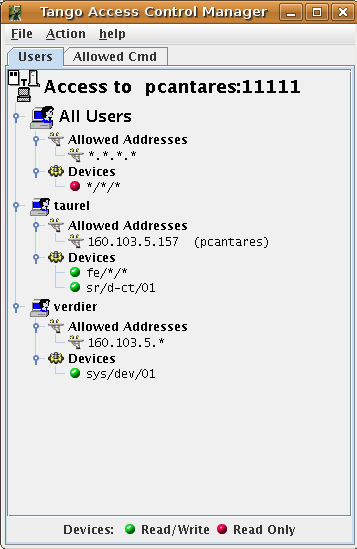
\includegraphics{advanced/control}\end{center}

In this example, the user \textquotedbl{}taurel\textquotedbl{} has
Write Access to the device \textquotedbl{}sr/d-ct/1\textquotedbl{}
and to all devices belonging to the domain \textquotedbl{}fe\textquotedbl{}
but only from the host \textquotedbl{}pcantares\textquotedbl{} He
has read access to all other devices but always only from the host
pcantares. The user \textquotedbl{}verdier\textquotedbl{} has write
access to the device \textquotedbl{}sys/dev/01\textquotedbl{} from
any host on the network \textquotedbl{}160.103.5\textquotedbl{} and
Read Access to all the remaining devices from the same network. All
the other users has only Read Access but from any host.


\subsection{Running a Tango control system with the controlled access}

All the users rights are stored in two tables of the Tango database.
A dedicated device server called \textbf{TangoAccessControl\index{TangoAccessControl}}
access these tables without using the classical Tango database server.
This TangoAccessControl device server must be configured with only
one device. The property \textbf{Services\index{Services} }belonging
to the free object\textbf{ CtrlSystem\index{CtrlSystem}} is used
to run a Tango control system with its controlled access. This property
is an array of string with each string describing the service(s) running
in the control system. For controlled access, the service name is
\textquotedbl{}AccessControl\textquotedbl{}. The service instance
name has to be defined as \textquotedbl{}tango\textquotedbl{}. The
device name associated with this service must be the name of the TangoAccessControl
server device. For instance, if the TangoAccessControl device server
device is named \emph{sys/access\_control/1}, one element of the Services
property of the CtrlSystem object has to be set to\begin{center}AccessControl/tango:sys/access\_control/1\end{center}

If the service is defined but without a valid device name corresponding
to the TangoAccessControl device server, all users from any host will
have write access (simulating a Tango control system without controlled
access). Note that this device server connects to the MySQL database
and therefore may need the MySQL connection related environment variables
MYSQL\_USER\index{MYSQL-USER} and MYSQL\_PASSWORD\index{MYSQL-PASSWORD}
described in \ref{sub:Db-Env-Variables}

Even if a controlled access system is running, it is possible to by-pass
it if, in the environment of the client application, the environment
variable SUPER\_TANGO\index{SUPER-TANGO} is defined to \textquotedbl{}true\textquotedbl{}.
If for one reason or another, the controlled access server is defined
but not accessible, the device right checked at that time will be
Read Access.\vspace{1cm}


\begin{center}
\label{FourRicardo}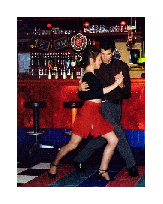
\includegraphics[scale=4]{dance/AT97-65-size}
\par\end{center}
